% NeurIPS 2026 main-track submission. Keep final/preprint disabled for review.
\documentclass{article}
\PassOptionsToPackage{numbers,sort&compress}{natbib}
\usepackage[main]{neurips_2026}
\usepackage[utf8]{inputenc}
\usepackage[T1]{fontenc}
\usepackage{graphicx}
\usepackage{amsmath}
\usepackage{amssymb}
\usepackage{booktabs}
\usepackage{multirow}
\usepackage{listings}
\usepackage{xcolor}
\usepackage{microtype}
\usepackage{url}
\usepackage[bookmarks=false,hidelinks]{hyperref}

\lstset{
  basicstyle=\ttfamily\small,
  breaklines=true,
  frame=single
}

% A little slack for long model IDs and feature labels.
\emergencystretch=1.5em

\renewcommand\UrlFont{\rmfamily}
\urlstyle{rm}

\title{Steering Tool Selection: Causal Evidence That Sparse Autoencoder Features Can Control Agent Decisions}

% The style suppresses this block in anonymous submission mode.
\author{%
  Hannes Hapke \\
  575 Lab, Dataiku Inc.\\
  Portland, OR, USA\\
  \texttt{hannes.hapke@dataiku.com}
  \And
  David Cardozo \\
  575 Lab, Dataiku Inc.\\
  Toronto, ON, Canada\\
  \texttt{david.cardozo@dataiku.com}
}

\begin{document}

\maketitle
\begin{abstract}
Sparse autoencoders (SAEs) can expose human-interpretable concepts in an
agent's activations, but naming a concept does not establish that it caused a
decision. We test this distinction by intervening on JumpReLU SAE features in
a 30B-parameter agent as it selects among tools. Using request pairs that
differ by a controlled cue, we ablate and cross-patch features at the decision
token while leaving the prompt unchanged. At late evaluated layers of this
model, a single feature in one case, and small cue-feature sets more broadly,
can redirect tool selection,
with effects substantially larger than those of mass-matched random controls
and reflected in generated responses. Measured against a dictionary-free
ceiling --- patching the whole residual at the same token --- those
interventions recover 29\% of the causal signal available there, and a dense
difference-in-means direction of equal magnitude recovers the same fraction, so
the sparse basis buys nameability rather than causal precision. The same cues are represented at
earlier layers, but of 460 interventions there only one flips a tool
selection, revealing a separation between where decision-relevant information is
readable and where it becomes causally effective. We also identify a failure
mode in which a nearly collapsed SAE dictionary attains the highest explained
variance in our study while providing an unusable causal decomposition. To
detect this failure, we propose comparing cross-patch and ablation effects as
an intervention-native diagnostic of dictionary utility. These results show
that feature interpretability, reconstruction quality, and causal relevance
must be evaluated separately when using SAEs to explain agent decisions.
\end{abstract}
%
\section{Introduction}
\label{sec:intro}

An agent that reads a request and picks a tool makes a discrete, consequential choice. \emph{Track delivery performance of our local supplier} sends it to a supplier database; change one word to \emph{global} and it reaches for a shipment tracker instead. Something inside the model represents the difference. Sparse autoencoders are the standard instrument for finding out what~\cite{ref_bricken2023,cunningham2023sparseautoencodershighlyinterpretable}, and in prior work~\cite{ref_hapke2025} we used them to decompose tool-selection activations into labelled, human-readable features and to validate those labels with token-level fuzzing.

That work established that the features are \emph{describable}. It did not establish that they are \emph{decisive}. The gap matters in practice: an operator shown a decision report saying ``the agent weighed \emph{forecast framing} at 0.7'' will act on it as if the feature caused the choice. A feature that merely tracks a word in the prompt supports no such reading. Correlational feature analysis cannot tell the two apart, and the ablation experiment in our earlier work --- zeroing ten features out of roughly 668 active ones at layer 20 --- moved only about 10\% of predictions on its single significant contrast type, which is consistent with either a weak cause or a poor intervention.

This paper closes that gap with interventions instead of descriptions. The design rests on three choices:

\begin{enumerate}
\item \textbf{Minimal pairs chosen by rule, at scale.} Two requests that differ by one cue and get different tools isolate the cue. We sweep 377{,}626 supply-chain and 327{,}988 customer-support training pairs and select demonstration pairs by explicit predicates --- including a non-saturation gate requiring the weaker side's tool probability to remain below 0.8, a criterion not satisfied by some pairs used in our earlier work --- so that pair choice is auditable rather than curated.
\item \textbf{Intervene at the decision token, in both directions.} We ablate a side's cue features and, more informatively, \emph{cross-patch}: clamp the donor side's feature activations into the recipient's decision token while leaving the recipient's prompt exactly as written. A cross-patch that flips the tool cannot be explained by the prompt, because the prompt did not change.
\item \textbf{Controls that can fail.} Every intervention is matched against random feature sets of the same activation mass --- at the granularity of the single reported family, of the whole clamped set, and, for cross-patch, of the change the clamp actually realises on the recipient; every dose curve against the same controls at every scale; the cue features against paraphrases that carry the meaning without the word and keyword probes that carry the word without the meaning; and the decision-token probabilities against what the model actually writes when allowed to generate.
\end{enumerate}

\paragraph{Contributions.}
\begin{itemize}
\item \textbf{A single-feature causal example, with broader small-set evidence.} In one case, clamping one SAE feature into an unmodified request flips the agent's tool at the donor's natural activation level (Sect.~\ref{sec:single}). Across a 64-pair expanded sample, interventions on small cue-feature sets produce 68 directed flips in 128 ablation sides and 41 in 128 cross-patch directions at each scenario's most responsive layer, against 20 and 15 at a layer that was not selected. These are exact dependent counts on two scenarios in one model, not population rates (Sect.~\ref{sec:expanded}).
\item \textbf{A denominator for causal claims about SAE features.} Patching the whole residual at the same token bounds what any decomposition read there can do. Cue-set interventions recover 29\% of it and bulk ones 41\%; a dense difference-in-means direction at the same magnitude recovers 24\%, and random directions at that magnitude 0\%. We report recovery fractions rather than bare flip rates and recommend the practice (Sect.~\ref{sec:ceiling}).
\item \textbf{Causal leverage is concentrated late in the evaluated model.} Across all scenarios and samples, 460 interventions at layers 6, 13 and 20 yield one directed flip, while the same battery at the primary layers flips 137 of 324. These dependent counts describe this model--task grid rather than independent trials or a universal account of where models make decisions (Sect.~\ref{sec:depth}).
\item \textbf{A degeneracy diagnostic that reconstruction metrics miss.} We characterise a collapsed dictionary whose explained variance is the best in the study, and show that the cross-patch/ablation \emph{ratio} separates it, wherever the ratio is defined, while explained variance and feature labels do not (Sect.~\ref{sec:degeneracy}).
\item \textbf{An honest account of what the features track.} Keyword controls hold 9/12 and paraphrases 30/40, so the features follow a narrow sense of the cue rather than the token --- but not the concept in general (Sect.~\ref{sec:semantics}).
\end{itemize}

\section{Related Work}
\label{sec:related}

\paragraph{Sparse autoencoders.} SAEs recover sparse, more monosemantic directions from superposed representations~\cite{elhage2022toymodelssuperposition,ref_bricken2023,cunningham2023sparseautoencodershighlyinterpretable}. We use the JumpReLU variant~\cite{ref_rajamanoharan2024}, which replaces the soft $L_1$ penalty with a learned per-feature threshold and improves the sparsity/fidelity trade-off; Gated SAEs address the same shrinkage problem differently~\cite{rajamanoharan2024improvingdictionarylearninggated}. Large open SAE suites such as Gemma Scope~\cite{lieberum2024gemmascopeopensparse} have made layer-by-layer comparison routine, and scaling studies~\cite{gao2024scalingevaluatingsparseautoencoders} have made clear that reconstruction loss and $L_0$ alone are weak proxies for usefulness. Sect.~\ref{sec:degeneracy} gives a concrete case where they point the wrong way.

\paragraph{Causal interventions.} Activation patching and causal tracing localise behaviour by transplanting activations between runs~\cite{meng2022locatingeditingfactualassociations,wang2022interpretabilitywildcircuitindirect}, with known pitfalls in interpretation~\cite{heimersheim2024useinterpretactivationpatching}; automated circuit discovery scales the search~\cite{conmy2023automatedcircuitdiscoverymechanistic}. Our cross-patch is activation patching performed in the SAE basis at a single token, which is what makes the transplanted quantity nameable. Sparse feature circuits~\cite{marks2024sparsefeaturecircuitsdiscovering} likewise combine SAEs with causal graphs, at the level of a circuit rather than a single decision.

\paragraph{Steering.} Adding a direction to the residual stream to change behaviour is well established~\cite{turner2024steeringlanguagemodelsactivation,zou2025representationengineeringtopdownapproach}, and SAE features have been used as the steering basis at scale~\cite{templeton2024scaling}. Evaluations of whether SAE features are actually the right control surface have been mixed~\cite{makelov2024principledevaluationssparseautoencoders}. Our contribution is not a new steering method but a discipline for reading one: matched-mass controls, a dose curve, a generation check, and a degeneracy test, applied to a decision with a discrete, externally meaningful outcome --- which tool gets called.

\paragraph{Agent tool use.} Tool-augmented agents~\cite{schick2023toolformerlanguagemodelsteach,yao2023reactsynergizingreasoningacting} are usually analysed behaviourally. Tool selection is an unusually convenient target for mechanistic work: the output is a short, closed set of names, so ``did the intervention change the decision'' has an unambiguous answer.

\section{Method}
\label{sec:method}

\subsection{Setup}

The subject model is NVIDIA-\allowbreak Nemotron-\allowbreak 3.5-\allowbreak Nano-\allowbreak 30B-\allowbreak A3B (BF16), a 52-layer hybrid architecture interleaving Mamba-2, attention and mixture-of-experts blocks, with $d_{\text{model}} = 2688$. We use the released JumpReLU SAEs trained on its residual stream at layers 6, 13, 20, 27, 34 and 43, each with $d_{\text{sae}} = 10{,}752$ ($4\times$ expansion) and a target $L_0$ of 75. Those dictionaries are trained, without any contrastive signal, on decision-token activations from the same generated corpus the evaluation draws on --- the 1{,}574{,}523 of 2{,}011{,}672 generated pairs whose two sides call different tools, over five agent scenarios and 37 contrast types --- so they have seen this prompt distribution, and 136 of the 150 requests evaluated here appear in it verbatim (the exception is \emph{tool selection}, whose 14 requests come from a separate released split). Sect.~\ref{sec:heldout} checks the consequences on contrast types the dictionaries never saw.

Each scenario supplies a system prompt listing six tools and a user request. The assistant turn is prefilled with \texttt{I'll use the}; the next token position is the \emph{decision token}. We read the distribution over tools by mapping the next-token logits through a token-prefix tree over the tool names, disambiguating shared first tokens by a second token where required. All interventions act at this one position, through a forward pre-hook on the target layer: encode the residual vector with the SAE, modify feature activations, decode, and continue the forward pass.

Decisions and residuals are captured with vLLM; interventions run under HuggingFace \texttt{transformers}, so we verify agreement per prompt. Residual cosine similarity between backends is 0.999 (min 0.998) for supply chain and 0.998 (min 0.994) for customer support, with identical baseline tool choices on all 20 requests. Compute is modest: everything runs on a single 80\,GB NVIDIA H100, capture takes about two minutes per scenario, a full one-layer intervention battery (128 interventions plus their matched controls) about three, and all interventions reported in this paper amount to under two GPU-hours. The behavioural sweep that feeds pair selection, and the SAE training itself, preceded this work and required substantially more.\footnote{Code, run artefacts, selection rules, per-pair reports and the scripts that regenerate every number and figure in this paper are available, anonymized for review, at \url{https://anonymous.4open.science/r/ml-inspector-0651/}.}

\subsection{Minimal pairs, selected by rule}
\label{sec:pairs}

A cue analysis is only as good as its pairs. Ours are selected from a full sweep of the scenario's clean training pairs --- 377{,}626 scorable for supply chain and 327{,}988 for customer support --- by predicates fixed in advance. Of the supply-chain pairs, 145{,}604 (38.6\%) flip the tool at all and 49{,}488 survive the joint flip-and-saturation gate; for customer support, 206{,}120 flip. The gate is:

\begin{itemize}
\item the two sides get different tools, both with probability $\geq 0.6$ (\emph{flip});
\item the \emph{weaker} side sits below 0.8, so neither side is saturated;
\item content-word Jaccard overlap $\geq 0.7$ (supply chain) or $\geq 0.55$ (customer support, whose contrasts are rephrasings rather than word swaps), so the pair really is a one-cue edit;
\item no tool is named in the request;
\item at most one pair per contrast type and two per tool combination.
\end{itemize}

The non-saturation gate is the consequential one. The seven pairs published in our earlier work were chosen for interpretability of the contrast, and its two top-ranked pairs turned out to sit at $p = 1.00$ on both sides, where no intervention short of catastrophic has anywhere to move. We keep those seven pairs here as a comparison set (\emph{tool selection}, 14 sides) alongside the rule-selected \emph{supply chain} (4 pairs, 8 sides) and \emph{customer support} (6 pairs, 12 sides).

\paragraph{An expanded sample for rate estimation.} The demonstration pairs are few by design --- one per contrast type, each examined individually. To estimate flip \emph{rates} we additionally sample 32 pairs per scenario from the full gate-passing population (1{,}094 supply-chain and 1{,}616 customer-support pairs pass every predicate above except the one-per-contrast cap), uniformly at random under a cap of ten pairs per contrast type. The cap matters: the gated population is dominated by whichever contrast type the template generator wrote the most minimal variants of (uncapped, 29 of 32 supply-chain draws land on \emph{demand pull vs.\ push} and 28 of 32 customer-support draws on \emph{billing vs.\ technical}), and within-type pairs are near-duplicates, so an uncapped sample buys correlated copies of one contrast rather than evidence. The sampled pairs pass through the identical capture and intervention battery at the scenario's primary layer and one early layer, giving 64 ablation sides and 64 cross-patch directions per scenario; the seed and selection are shipped with the artefacts.

\paragraph{What the cap makes these rates mean.} The cap is a quota, so what it estimates is not a rate in the gated population. \emph{Demand pull vs.\ push} holds 1{,}006 of the 1{,}094 supply-chain pairs and \emph{billing vs.\ technical} 1{,}565 of the 1{,}616 customer-support pairs; capping at ten deliberately under-represents both. We therefore state the estimand as a \textbf{flip rate averaged over contrast types under a ten-pair quota}, not a rate in the gate population. Re-weighting the same interventions back to that population by stratum share moves them up rather than down --- pooled ablation 0.53 either way, cross-patch 0.32 quota against 0.46 weighted --- so the quota is not flattering the headline.\footnote{Per scenario, population-weighted against quota: supply chain 0.61/0.63 ablation and 0.53/0.36 cross-patch; customer support 0.45/0.44 and 0.39/0.28. The weighted estimator (Horvitz--Thompson, contrast type as stratum) carries an effective $n$ of 21--24 rather than 64, because 92--97\% of the population weight sits on one stratum sampled with ten pairs --- exactly the concentration the cap exists to avoid. Stratum counts and the estimator are in the released report.}

Two contrast types are absent from supply chain by construction: across roughly 10{,}000 qualifying pairs each, \emph{spot buy vs.\ contract} peaks at Jaccard 0.47 and \emph{just-in-time vs.\ safety stock} at 0.36. Their contrast is written as structurally different sentences, so no one-cue pair exists at any threshold, and the selector drops them rather than quietly relaxing the gate.

Table~\ref{tab:pairs} shows the supply-chain set. The first pair is the sharpest available test: side A contains \emph{no cue token at all}, so on that side there is no lexical anchor for a feature to latch onto.

\begin{table}[t]
\caption{The rule-selected supply-chain pairs. $J$ is content-word Jaccard overlap; $p$ is the sweep's decision-token probability for that side's tool. Tools are named by their distinguishing word: \texttt{inventory\_manager}, \texttt{demand\_forecaster}, \texttt{supplier\_database}, \texttt{shipment\_tracker}, \texttt{route\_optimizer}.}
\label{tab:pairs}
\centering
\footnotesize
\setlength{\tabcolsep}{4pt}
\begin{tabular}{@{}llrlrlr@{}}
\toprule
& & & \multicolumn{2}{c}{Side A} & \multicolumn{2}{c}{Side B} \\
\cmidrule(lr){4-5}\cmidrule(lr){6-7}
Contrast type & Cue (A / B) & $J$ & Tool & $p$ & Tool & $p$ \\
\midrule
demand pull/push & \emph{(none)} / \emph{forecasted} & 0.88 & inventory & 0.98 & forecaster & 0.80 \\
local/global & \emph{local} / \emph{global} & 0.82 & supplier & 0.95 & shipment & 0.80 \\
cost/speed & \emph{economical} / \emph{express} & 0.78 & route & 0.83 & shipment & 0.79 \\
single/multi source & \emph{our main} / \emph{all} & 0.70 & supplier & 0.71 & inventory & 0.83 \\
\bottomrule
\end{tabular}
\end{table}

\subsection{Interventions}

For a pair $(A, B)$ we take each side's \emph{cue families}: the features active at that side's decision token whose activation differs materially across the pair, grouped into families where a group of indices behaves as one unit. Typical family counts are 3--14 features per side. We then run three interventions.

\paragraph{Ablation.} Set side $X$'s cue families to zero at $X$'s own decision token and re-read the tool distribution. This asks whether the cue is \emph{necessary}.

\paragraph{Cross-patch.} Clamp side $X$'s cue-family activations, at the values they take on $X$'s request, into side $Y$'s decision token --- with $Y$'s prompt unchanged. This asks whether the cue is \emph{sufficient}. We run two variants: \textsc{cue}, which clamps only the cue families, and \textsc{bulk}, which clamps every feature active on the donor. The distinction is central to Sect.~\ref{sec:degeneracy}: \textsc{bulk} on a sparse layer is a modest superset of \textsc{cue}, but on a dense layer it transplants the entire representation and stops being an interpretability result.

\paragraph{Dose-response.} Repeat the cross-patch at scales $\{0, 0.5, 1, 1.5, 2, 3\} \times$ the donor's activation. Scale $1$ is the natural operating point; a curve that only crosses at $3\times$ is telling us about saturation, not about the feature.

\subsection{Controls and the definition of a flip}

We call an intervention a \textbf{directed flip} when the argmax over tools changes \emph{and} lands on the donor's (or, for ablation, the other side's) tool. An intervention that knocks the model onto some third tool is disruption, not steering, and we do not count it. The looser any-tool count is also recorded in the released report; the two disagree in 5 of the 36 cells of the depth grid, never by more than two flips, and in four of the five it is an ablation that knocked the model onto a third tool. For ablation this criterion is weaker than it looks, because on a minimal pair the other side's tool is usually the baseline runner-up, so an intervention that merely degrades the winner produces a directed flip by default; Sect.~\ref{sec:expanded} reports the full outcome partition and audits that confound.

Four controls guard the readings:

\begin{description}
\item[Mass-matched random features.] Three families of random control sets, each drawn from the features active on the intervened prompt, each with three draws, each contributing the largest $|\Delta p|$ it produces as a band. \textsc{Per-family} matches every intervened feature family on its own activation mass and count, and is the band for a single reported row. \textsc{Set-matched} matches the \emph{whole} cue set on total mass and count, and is the band for a set-level claim; the distinction is not cosmetic, since a cue set carries a median $2.15\times$ the mass of the heaviest per-family draw on the demonstration sets and $1.72\times$ on the expanded sample. \textsc{Difference-matched} answers a third question, and it is the one the selection rule forces: cue families are chosen \emph{because} they differ across the pair, so a control matched only on mass asks whether removing that much activation matters, not whether removing the \emph{differing} activation matters. Both arms therefore get draws matched on $\sum_i \lvert v^{X}_i - v^{Y}_i \rvert$ over the two sides of the pair, excluding the cue set: for cross-patch that quantity is also the change the clamp realises on the recipient (donor mass overstates it whenever a feature is already active there), and for ablation it is how much the drawn set distinguishes the two requests. Draws accumulate features until they reach the target, so a matched draw always carries at least the intervened set's mass (median $1.04\times$, never below $1.00\times$ over the 882 set-matched draws), and the comparison is conservative in the intended direction. When the eligible pool cannot reach the target at all we draw the whole pool, mark the draw as unmatched --- a \emph{ceiling} --- and keep those sides out of the matched comparisons; this happens on 30 of 324 sides.
\item[Keyword probes.] The other side's request with this side's cue word inserted in a semantically inert role (\emph{``\dots using the cost codes from the \textbf{forecasted} budget approved last week''}). A feature that tracks meaning should leave the decision alone.
\item[Paraphrases.] This side's request restated without any of its cue words. A feature that tracks meaning should still fire, and the tool should not move.
\item[Generation.] Beyond the decision token, we let the model write 48 tokens under the steered activations, under the baseline, and under a $\Delta$-matched random control drawn from the recipient's own active features, and compare which tool it names. We run this twice: clamping at every position, and clamping at the decision token alone, which is the same single-position intervention the rest of the paper reports.
\end{description}

\paragraph{Statistical treatment.} Generated pairs within a contrast type are near-duplicates, and the two intervention directions of a pair are dependent. We therefore resample whole clusters for the expanded sample: the unit is a contrast type within a scenario, all pairs and directions in a drawn cluster are retained, and the draws are stratified within scenario, since pooling the clusters would let a resample vary a scenario mix the design held constant. Clusters are unequal in size, so this fixes the number of clusters each scenario contributes rather than the number of pairs; averaging per-scenario rates with equal weights, which fixes the latter, gives 0.43--0.65 and 0.17--0.49. The distribution is enumerated exactly rather than sampled --- 35 count vectors for supply chain's four clusters and 462 for customer support's six, 16{,}170 together, each weighted by the ordered draws producing it --- so the endpoints carry no seed dependence. Pooling all ten instead widens ablation to 0.40--0.66 and leaves cross-patch at 0.16--0.48. At that cluster count a percentile bootstrap is anti-conservative, so we read the brackets as a floor on the uncertainty rather than a 95\% guarantee, and treat the exact dependent counts as the result throughout. Per-scenario and demonstration results are reported as exact counts rather than population-rate estimates. Cue interventions are also compared directly with their stored mass-matched controls --- set-level effects against the \textsc{set-matched} family, cross-patch additionally against the $\Delta$-matched one --- with the matched sides and the ceiling sides counted separately. We report those paired counts descriptively rather than attach tests that would treat clustered interventions as independent; the exact exchangeability and sign statistics on the matched subsets are released with the report and carry that same dependence. The bootstrap is implemented in the released \texttt{extract\_results.py}.

\section{Results}
\label{sec:results}

\subsection{A single-feature case study}
\label{sec:single}

Take the sharpest pair. Side B reads \emph{``Adjust inventory for items with rising forecasted customer order frequency''}, and the agent calls \texttt{demand\_forecaster} with $p = 0.85$, leaving $p(\texttt{inventory\_manager}) = 0.15$. Side A is the same sentence without \emph{forecasted}, and the agent calls \texttt{inventory\_manager}.

At layer 43 we clamp a single feature --- index 2101, labelled \emph{``safety stock and inventory coverage calculation''} --- from side A into side B's decision token. B's prompt is untouched; it still says \emph{forecasted}. The tool changes to \texttt{inventory\_manager}, with $p$ rising from 0.15 to 0.71. All six cue families together give 0.73, so this one feature carries essentially the whole effect. Three random sets matched on feature 2101's own activation move $p$ by at most 0.03; three matched on the whole cue set --- 56.1 of activation mass across six features, against 34.2 for the heaviest single-family draw --- move it by at most 0.05.

Figure~\ref{fig:dose} shows the dose curve. It crosses 0.5 between $0.5\times$ and $1\times$ and is already past it at the donor's natural activation --- the feature does not need to be amplified beyond what the model itself produces when the request genuinely lacks the word \emph{forecasted}. The control band is wide at scale~0, where zeroing a mass-matched random set is itself disruptive, and narrow from $0.5\times$ on, where the steered curves are far outside it.

\begin{figure}[t]
\centering
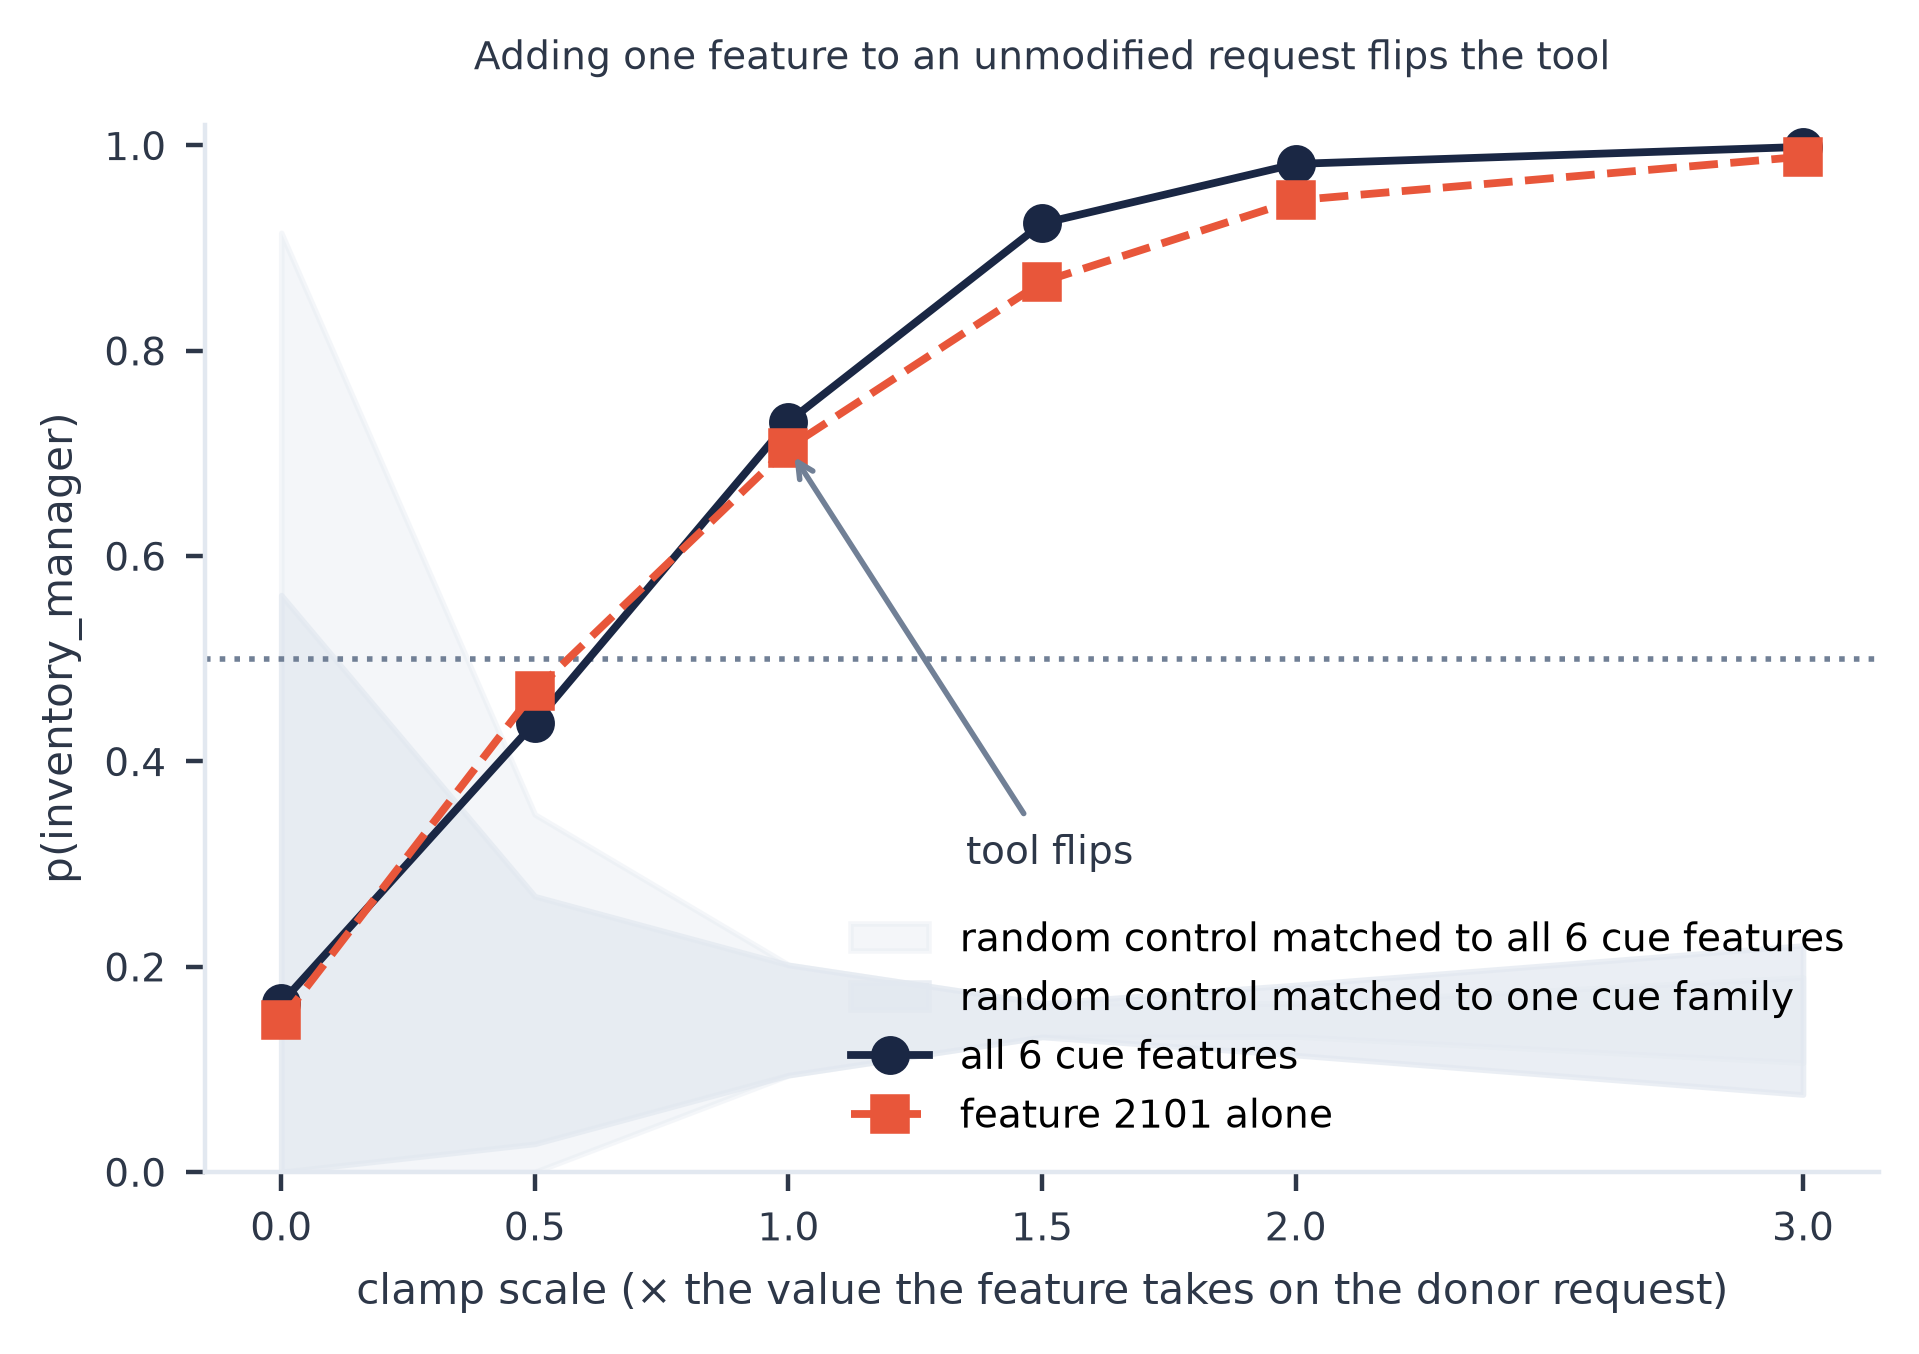
\includegraphics[width=0.86\textwidth]{images/chart_dose.png}
\caption{Cross-patching feature 2101 from side A into side B's unmodified request. Shaded: the largest deviation produced by three random feature sets at the same scale, matched to the intervened family (dark) and to the whole cue set (light). The curve crosses $p = 0.5$ at the donor's natural activation ($1\times$), and one feature accounts for nearly all of what the full cue set does.}
\label{fig:dose}
\end{figure}

The expanded sample does not establish that single-feature steering is typical: feature 2101 is our clearest single-feature case. It does show that causal effects from the broader cue-feature sets are not confined to that pair. At layer 43, ablating a side's cue families flips 7 of 8 evaluated supply-chain sides, with $|\Delta p|$ up to 0.85 against set-matched control bands of 0.03--0.19; the five largest beat those bands by 6--25$\times$, though on two of them the cue set outweighs every other active feature combined, so the control is the whole eligible pool rather than a matched draw. Three of eight cross-patch directions flip, all three driven by the cue families rather than by bulk transplant. Customer support, read at layer 34, flips 6 of 12 sides under ablation and 4 of 12 cross-patch directions. These are exact counts on small, dependent demonstration sets, not estimated rates; rate estimation is deferred to the expanded sample below.

The matched controls provide a descriptive comparison on the same requests. Against the \textsc{set-matched} family --- drawn to the mass and count of the whole clamped set --- the cue set exceeds the \emph{maximum} $|\Delta p|$ of its three draws on 33 of 34 ablation sides (30 of the 31 genuinely matched, and all 3 ceilings) and 28 of 34 cross-patch directions (25 of 31 matched, 3 of 3 ceilings). Matching instead on the change the clamp realises leaves cross-patch at 27 of 34, but 11 of the 34 are ceilings: the cue set moves a median 0.71 of the donor's activation mass, and frequently no other set of active features can move as much. At feature-family granularity, individual cue families change the recipient's tool in 5 of 204 rows --- 4 of them onto the donor's tool --- while none of the 816 control draws stored across the three families does. These comparisons show a consistent separation on the evaluated cases, but their clustered rows should not be read as independent trials.

\paragraph{The model writes it, too.} Allowed to generate 48 tokens with the clamp held at the decision token alone --- the same one-position intervention as everything above --- 13 of 20 continuations are byte-identical to the baseline, and of the 7 that change, 5 name the donor's tool as their first tool. Clamping instead at every position, a far larger intervention, gives 6 of 20; the two counts share 4 directions, so the bigger intervention is not simply the stronger one. No $\Delta$-matched control follows in either arm (0 of 20). The denominator deserves care: only 5 of those 20 directions have their decision-token argmax flipped by the cue set at all, and those 5 are exactly the 5 whose text names the donor's tool. Every decision-token flip in this set persisted into 48 tokens of generation, and no continuation named the donor's tool without the argmax having moved first. Five flips bound very little, but the relevant conditional is 5 of 5, not 5 of 20. One example, from a prompt that was never edited and 7 activations clamped at the decision token:

\begin{quote}\small
\textbf{baseline:} \texttt{shipment\_tracker} tool to analyze the delivery performance of your global electronic components supplier over the last quarter\dots\\
\textbf{steered:} supplier database to look up information about your global electronic components supplier and their delivery performance\dots\\
\textbf{control:} byte-identical to baseline
\end{quote}

\noindent The control here is a ceiling draw, and an instructive one: the 16 features it takes from the recipient's own activation move a total of 7.5, against the 36.3 the cue set moves. On this direction no set of other active features can be found that does as much, which is a fact about the cue set rather than a weakness of the control.

We treat these as confirmation rather than independent evidence: each had already crossed 0.5 in its dose curve. Their value is in ruling out that the effect lives only in a next-token readout that never reaches behaviour --- and, since the decision-token arm changes nothing at all on 13 of 20 prompts and changes the tool on 5 of the remaining 7, in showing that a clamp at one position is usually inert and rarely disruptive when it is not.

\subsection{Flip rates on the expanded sample}
\label{sec:expanded}

The demonstration pairs establish existence; the expanded sample of Sect.~\ref{sec:pairs} gives counts on a larger, rule-selected set. Table~\ref{tab:expanded} gives the result at three layers. At the selected layers, ablation flips 68 of 128 sides and cross-patch 41 of 128 directions, 29 of the 41 driven by the cue families alone; at layer 27, which no selection step touched, the same pairs give 20 of 128 and 15 of 128. A contrast-cluster bootstrap over the ten scenario-by-contrast clusters puts the selected-layer rates at 0.53 [0.42, 0.66] and 0.32 [0.16, 0.48], but with only ten clusters a percentile bootstrap is expected to \emph{under}-cover, so we read those brackets as a floor on the uncertainty and treat the counts, not the rates, as the result. Backend parity holds on all 128 fresh prompts (mean residual cosine 0.999 supply chain, 0.998 customer support), and the captured baseline tool matches the sweep's on 128 of 128 sides.

\paragraph{Where the argmax goes.} A directed flip requires the new argmax to be the paired tool, so the full partition matters (Table~\ref{tab:outcomes}). It is favourable for cross-patch and awkward for ablation. Cross-patching the cue families leaves the tool unchanged on 96 of 128 directions, moves it to the donor's tool on 29, and to some third tool on 3; the 3{,}057 stored control draws move it to the donor's tool 27 times (0.9\%) and to a third tool 15 times. Ablation leaves the tool unchanged on 47 of 128 sides, moves it to the paired tool on 68, and to a third tool on 13.

The awkwardness is that the paired tool is usually where a merely destructive ablation would land anyway. Because the gate selects two near-identical prompts that take different tools, \textbf{the paired tool is the baseline runner-up on 91 of the 128 sides}, and 75 of the 81 ablation flips land on the baseline runner-up whatever it happens to be. Splitting on that: where the paired tool is the runner-up, all 63 flips land on it; where it is not, only 5 of 18 do. So for ablation the directed criterion adds little beyond ``the argmax moved'', and 68 of 128 is better read as 81 of 128 argmax changes whose destination is largely fixed by the pair. We report the ablation arm on that basis. What the confound does \emph{not} explain is whether a flip happens at all, and the controls settle that, because they are drawn on the same prompts and inherit the same runner-up structure. Of the 3{,}057 stored ablation control draws, 3{,}032 leave the tool untouched; 6 move it to the paired tool and 19 to a third tool. So a mass- or difference-matched ablation of the same size changes the decision on 0.8\% of draws where the cue set changes it on 63\%, and lands on the paired tool on 0.2\% where the cue set does on 53\%. The cross-patch controls behave the same way (27 directed and 15 third-tool in 3{,}057). We read the ablation arm accordingly: the runner-up structure governs \emph{where} a flip goes, and the controls show it does not govern \emph{whether} one happens.

\begin{table}[t]
\caption{Full outcome partition on the expanded sample, and the runner-up audit for ablation. ``Third tool'' is an argmax change that lands on neither side's tool. Control rows cover every stored draw across the three matching families of each arm, on the same prompts and with the same runner-up structure as the interventions above them.}
\label{tab:outcomes}
\centering
\small
\setlength{\tabcolsep}{6pt}
\begin{tabular}{@{}lcccc@{}}
\toprule
Intervention & $n$ & unchanged & directed & third tool \\
\midrule
Ablation (cue families)      & 128  & 47   & 68 & 13 \\
Cross-patch (\textsc{cue})    & 128  & 96   & 29 & 3 \\
Cross-patch (\textsc{bulk})   & 128  & 83   & 41 & 4 \\
Ablation controls            & 3{,}057 & 3{,}032 & 6  & 19 \\
Cross-patch controls         & 3{,}057 & 3{,}015 & 27 & 15 \\
\midrule
\multicolumn{5}{@{}l@{}}{\emph{Ablation runner-up audit}: paired tool is the baseline runner-up on 91/128 sides;} \\
\multicolumn{5}{@{}l@{}}{75 of 81 flips land on the baseline runner-up; 63/63 when it is the paired tool, 5/18 when it is not.} \\
\bottomrule
\end{tabular}
\end{table}

\begin{table}[t]
\caption{Directed flips on the expanded sample --- 32 pairs per scenario, the same pairs at every layer. $\star$ marks each scenario's primary layer, which was selected as the most responsive of the six in Table~\ref{tab:depth}; layers 13 and 27 were not selected on anything. Rates are averaged over contrast types under the ten-pair quota of Sect.~\ref{sec:pairs}, not rates in the gate population, and they are exact dependent counts rather than population estimates. The cross-patch split counts flips driven by cue families alone (\textsc{cue}) versus those needing every donor-active feature (\textsc{bulk}).}
\label{tab:expanded}
\centering
\small
\setlength{\tabcolsep}{5pt}
\begin{tabular}{@{}llcccc@{}}
\toprule
& & \multicolumn{2}{c}{Ablation} & \multicolumn{2}{c}{Cross-patch} \\
\cmidrule(lr){3-4}\cmidrule(lr){5-6}
Scenario & Layer & flips & rate & flips (\textsc{cue}+\textsc{bulk}) & rate \\
\midrule
Supply chain     & 13          & 0/64           & 0.00 & 0/64          & 0.00 \\
                 & 27          & 11/64          & 0.17 & 6/64 (4+2)    & 0.09 \\
                 & 43$^{\star}$ & \textbf{40/64} & 0.63 & \textbf{23/64} (16+7) & 0.36 \\
\addlinespace
Customer support & 13          & 1/64           & 0.02 & 0/64          & 0.00 \\
                 & 27          & 9/64           & 0.14 & 9/64 (6+3)    & 0.14 \\
                 & 34$^{\star}$ & \textbf{28/64} & 0.44 & \textbf{18/64} (13+5) & 0.28 \\
\bottomrule
\end{tabular}
\end{table}

Against the set-matched controls, the cue set exceeds the maximum of its three draws on 118 of 128 ablation sides (103 of the 113 genuinely matched, and all 15 ceilings) and 104 of 128 cross-patch directions (92 of 113 matched, 12 of 15 ceilings). Matching on the realised change gives 105 of 128 for cross-patch, but here the ceiling problem is severe: on 68 of the 128 directions no set of other active features can move as much as the cue set does, since the cue set moves a median 0.52 of the donor's mass. That is a real limit on how tight a control can be made at this granularity, and we report it rather than quoting only the matched subset.

One thing changes from the demonstration sets, and it is worth reporting: the controls are no longer perfectly silent. Thirteen of 384 set-matched draws and 14 of 384 $\Delta$-matched draws change the recipient's tool (3.4\% and 3.6\%), against 41 of 128 cue-set cross-patches (32\%); at row level, 15 of 2{,}289 per-family draws (0.7\%) do, against 23 of 763 single cue families (3.0\%). The expanded pairs sit near the decision boundary by construction --- the gate requires the weaker side below 0.8 --- so a random mass-matched perturbation can occasionally tip a near-tied baseline. These are paired descriptive comparisons; clustered resampling, rather than a row-level test, supplies uncertainty for the pooled flip rates.

\paragraph{A second draw, and a layer nobody selected.} Two checks bound how much of Table~\ref{tab:expanded} is the particular sample and the particular layer. Redrawing 32 pairs per scenario under the same rule with a different seed gives 69 of 128 ablation flips (0.54, against 0.53) and 33 of 128 cross-patch (0.26, against 0.32); we report the seeds separately rather than pooling, since the second was drawn after the first was analysed. Running the original 128 pairs at layer 27 --- a layer no selection step ever touched --- gives 20 of 128 ablation (0.16, [0.09, 0.22]) and 15 of 128 cross-patch (0.12, [0.04, 0.20]). The primary-layer rates are thus $3.4\times$ and $2.7\times$ a non-selected late layer, with the ablation intervals not overlapping; Sect.~\ref{sec:limitations} takes up what the selection buys.

These counts have no denominator on their own; Sect.~\ref{sec:ceiling} supplies one.

\paragraph{Cue-ness or mass?} Cue families are selected for differing across the pair, so the difference-matched family is the control that tests the selection rule rather than the intervention size. It divides the 128 ablation sides in two. On 65 of them no set of other active features differs across the pair as much as the cue set does, so the draw is a ceiling --- which is itself the answer, and the strong form of it: on those sides the differing features essentially \emph{are} the cue features. The cue set exceeds that ceiling on 60 of the 65. On the 63 sides where a genuinely difference-matched control exists, the cue set exceeds it on 57. The demonstration sets give 10 ceilings and 24 matched sides, with 10 and 21 exceedances. No side had an empty pool, so the comparison was always made.

We report the six matched sides where it fails, because they are the cases the objection describes. Five of them are sides where the cue set does little in the first place --- $|\Delta p|$ of 0.008 to 0.335 with no flip --- so what the comparison records is that a difference-matched draw was not beaten by an ablation that barely moved anything. The sixth is the one that matters: \emph{single vs.\ multi source} side A, where the cue set moves $|\Delta p| = 0.281$ and \emph{does} flip the tool, against a difference-matched band of 0.292. There, a random set that distinguishes the two requests as well as the cue set does moves the decision just as far, and we do not claim that side as evidence. One such side in 63 is the honest summary.

\paragraph{What the quota averages over.} Contrast types differ enough that a pooled rate conceals the shape of the result. Ablation, by type: supply chain 12/20 (\emph{demand pull vs.\ push}), 16/20 (\emph{local vs.\ global}), 9/20 (\emph{cost vs.\ speed}), 3/4 (\emph{single vs.\ multi source}); customer support 9/20, 10/20, 2/14, 4/6, 1/2, 2/2. Cross-patch, same order: 11/20, 9/20, \textbf{0/20}, 3/4; and 8/20, 1/20, 4/14, 3/6, 0/2, 2/2. The one type that contributes no cross-patch flip at all is \emph{cost vs.\ speed}, independently flagged as the weak pair in Sect.~\ref{sec:limitations} --- and it holds 3.0\% of the gated supply-chain population while the cap gives it ten of the 32 sampled pairs, so the quota weights it about thirty times more heavily than the population does.

\subsection{How much of the decision token's causal signal is this?}
\label{sec:ceiling}

A flip count has no denominator. Twenty-nine of 128 cross-patch directions is a large number if little else at that token would move the decision and a small one if almost anything would, and nothing above distinguishes those cases. We therefore ran three references with no dictionary anywhere in the path (Table~\ref{tab:ceiling}).

\paragraph{The ceiling.} Replace the recipient's residual at the decision token with the donor's --- ordinary activation patching in the model's own basis. Whatever causal signal that position carries, this moves all of it, so no decomposition read there can beat it. It flips 100 of 128 expanded directions and 30 of 34 demonstration directions.

How much is available differs by setting, which is itself worth reporting: supply chain at layer 43 gives 61 of 64, customer support at layer 34 only 39 of 64. On the 25 customer-support directions where even a full transplant does not change the tool, $p$(donor's tool) still moves a long way without crossing --- 0.04 to 0.47 in one case --- so the decision there is partly re-derived downstream from the recipient's own context rather than settled at the position we intervene on. Normalising by the ceiling reverses which scenario looks better: the cue set flips 16 of 64 supply-chain directions and 13 of 64 customer-support ones (0.25 and 0.20), but recovers 0.26 and \emph{0.33} of what is available at the respective positions. Customer support looks weaker only because less of its decision is settled where we intervene.

\paragraph{A direction that needs no dictionary.} The mean (side A $-$ side B) residual of the \emph{other} pairs of the same contrast type, added to the recipient: no per-pair activations, no dictionary, and nothing to read off it. At the norm of this pair's own donor-minus-recipient difference it flips 79 of 124, far more than either SAE arm.

That comparison is not size-matched, and the size turns out to be all of it. Re-running the same direction at the norm of the cue clamp's own residual change --- reconstructed from the battery's stored targets as $\sum_i \gamma\,(v^{\text{target}}_i - v^{\text{current}}_i)\,W_{\text{dec}}[i]$, the change the delta hook actually applies --- gives 30 of 124, against the cue set's 29 of 128. The two are indistinguishable. The sparse basis therefore costs nothing in effectiveness against a dense direction of equal magnitude; what separates both from the ceiling is how much of the residual they move, not which basis they move it in. Random directions confirm that neither is a magnitude artefact: 2 of 384 at the full difference norm and 0 of 372 at the clamp norm.

\paragraph{What this does to the claim.} Cue-feature interventions recover \textbf{29\% of the causal signal available at the decision token}, and clamping every donor-active feature recovers 41\%. We think a recovery fraction, not a flip rate, is the honest headline for work of this kind, and we would not have known ours without running the ceiling. It does not weaken the causal reading of any individual intervention, and it does not favour the dense alternative: at equal size the two are the same, and only one of them says what it changed.

\begin{table}[t]
\caption{Every intervention at the decision token, ordered by effect. \emph{Basis} is what the intervention is expressed in: the model's residual stream, or the SAE dictionary. The two norms are the pair's full donor-minus-recipient difference and the smaller change the cue-set clamp itself makes. Difference-in-means needs several pairs per contrast type and so is undefined on the demonstration sets; four expanded directions lack it for the same reason.}
\label{tab:ceiling}
\centering
\small
\setlength{\tabcolsep}{5pt}
\begin{tabular}{@{}llcccc@{}}
\toprule
& & \multicolumn{2}{c}{Demonstration} & \multicolumn{2}{c}{Expanded} \\
\cmidrule(lr){3-4}\cmidrule(lr){5-6}
Intervention & Basis & flips & rate & flips & rate \\
\midrule
Full residual patch (ceiling)        & model & 30/34 & 0.88 & 100/128 & 0.78 \\
Difference-in-means, difference norm & model & ---   & ---  & 79/124  & 0.64 \\
All donor-active features (\textsc{bulk}) & SAE & 12/34 & 0.35 & 41/128  & 0.32 \\
Difference-in-means, clamp norm      & model & ---   & ---  & 30/124  & 0.24 \\
Cue set (\textsc{cue})               & SAE   & 7/34  & 0.21 & 29/128  & 0.23 \\
Random direction, difference norm    & model & 1/102 & 0.01 & 2/384   & 0.01 \\
Random direction, clamp norm         & model & ---   & ---  & 0/372   & 0.00 \\
\midrule
\multicolumn{2}{@{}l}{\emph{Recovery}: cue set / ceiling} & \multicolumn{2}{c}{0.23} & \multicolumn{2}{c}{0.29} \\
\multicolumn{2}{@{}l}{\hphantom{\emph{Recovery}: }\textsc{bulk} / ceiling} & \multicolumn{2}{c}{0.40} & \multicolumn{2}{c}{0.41} \\
\bottomrule
\end{tabular}
\end{table}

\subsection{A held-out check on unseen contrast types}
\label{sec:heldout}

The dictionaries were fitted on the corpus these pairs come from (Sect.~\ref{sec:method}), so the rates above are in-distribution. To ask how much of the effect depends on that, we wrote fresh request pairs along eight contrast axes that appear nowhere in the training corpus --- for supply chain, \emph{warehouse vs.\ transit capacity}, \emph{vendor defect vs.\ pricing record}, \emph{recorded vs.\ projected consumption}, \emph{carrier distance vs.\ carrier price}; for customer support, \emph{published spec vs.\ how-to}, \emph{prior orders vs.\ open invoice}, \emph{many reporters vs.\ one}, \emph{warranty coverage vs.\ repair guidance}. None of the 192 resulting requests occurs among the corpus's 2.0M pairs, and none of the eight axes is one of its 37 contrast types. Each pair is a single content-word swap, so it meets the same Jaccard requirement without relaxing it, and the pairs pass through the same sweep, the same gate and the same battery at the scenario's primary layer.

Of 96 authored pairs, 15 clear the gate (8 supply chain, 7 customer support), giving 30 sides and 30 directions. Ablation flips 9 of 30 (0.30, Wilson 0.17--0.48) and cross-patch 7 of 30 (0.23, 0.12--0.41), against 0.53 and 0.32 on the in-distribution sample. The intervals are wide and overlap, so we do not read a rate difference from 15 pairs --- and the cross-patch comparison is closer than those two figures suggest, because all 7 held-out flips come from the cue families while 12 of the in-distribution 41 need every donor-active feature. Cue-driven against cue-driven, the two are 0.23 and 0.23.

The per-intervention effect does not shrink. Measured as the cue set's $|\Delta p|$ against that side's own set-matched control band --- a quantity that does not depend on where the argmax boundary sits --- the median is $4.60\times$ on the held-out supply-chain sides against $2.72\times$ in distribution, and $5.30\times$ against $7.24\times$ for customer support; 71\% and 96\% of held-out sides exceed their own control band, against 78\% and 95\%. What differs is how often the argmax crosses: several held-out sides move $p$ by 0.3--0.5 at 5--13$\times$ their control band without changing the tool, because their baselines are more lopsided.

\paragraph{The same share of a comparable ceiling.} Flip rates alone cannot separate ``the features are weaker here'' from ``less of the decision is available here'', so we ran the ceiling of Sect.~\ref{sec:ceiling} on the held-out pairs too. It flips 25 of 30, a slightly \emph{higher} share than the 100 of 128 in distribution, so the held-out prompts are not ones where the decision token carries less. Against that denominator the cue set recovers \textbf{0.28} of the available signal, against 0.29 in distribution. Difference-in-means at the cue clamp's norm recovers 7 of 28 and random directions 0 of 84, the same ordering as in distribution. The one figure that does drop is the bulk arm, 0.28 against 0.41, and for a legible reason: no held-out flip required clamping beyond the cue families.

We report this as a probe, not a second rate estimate: we chose the axes and wrote the sentences, so the denominator reflects our drafting rather than a population. What it addresses is the narrower question of whether the effects above require the dictionary to have been fitted on the very prompts being intervened on. On prompts and contrast axes it never saw, cue-feature interventions move the decision as far outside their controls as they do in distribution, and recover the same share of what is causally available at the decision token.

\subsection{In this model, causal leverage is late while description is early}
\label{sec:depth}

We ran the full ablation and cross-patch battery at all six SAE layers for all three scenarios: 18 runs covering 34 ablation sides and 34 cross-patch directions per layer, 408 interventions in all. Table~\ref{tab:depth} and Fig.~\ref{fig:depth} give the result.

\begin{table}[t]
\caption{Directed flips at every SAE layer: cross-patch directions $\cdot$ ablation sides. Layers 6--20 produce none at all. The starred cell is an artefact of a collapsed dictionary, not a strong result (Sect.~\ref{sec:degeneracy}).}
\label{tab:depth}
\centering
\small
\setlength{\tabcolsep}{9pt}
\begin{tabular}{@{}lccc@{}}
\toprule
Layer & Tool selection & Supply chain & Customer support \\
& (7 pairs) & (4 pairs) & (6 pairs) \\
\midrule
6  & 0/14 $\cdot$ 0/14 & 0/8 $\cdot$ 0/8 & 0/12 $\cdot$ 0/12 \\
13 & 0/14 $\cdot$ 0/14 & 0/8 $\cdot$ 0/8 & 0/12 $\cdot$ 0/12 \\
20 & 0/14 $\cdot$ 0/14 & 0/8 $\cdot$ 0/8 & 0/12 $\cdot$ 0/12 \\
27 & 1/14 $\cdot$ 0/14 & 0/8 $\cdot$ 0/8 & 1/12 $\cdot$ 1/12 \\
34 & 2/14 $\cdot$ 0/14 & 2/8 $\cdot$ 1/8 & \textbf{4/12 $\cdot$ 6/12} \\
43 & \textbf{5/14 $\cdot$ 3/14} & \textbf{3/8 $\cdot$ 7/8} & 9/12$^{\star}$ $\cdot$ 1/12 \\
\bottomrule
\end{tabular}
\end{table}

\begin{figure}[t]
\centering
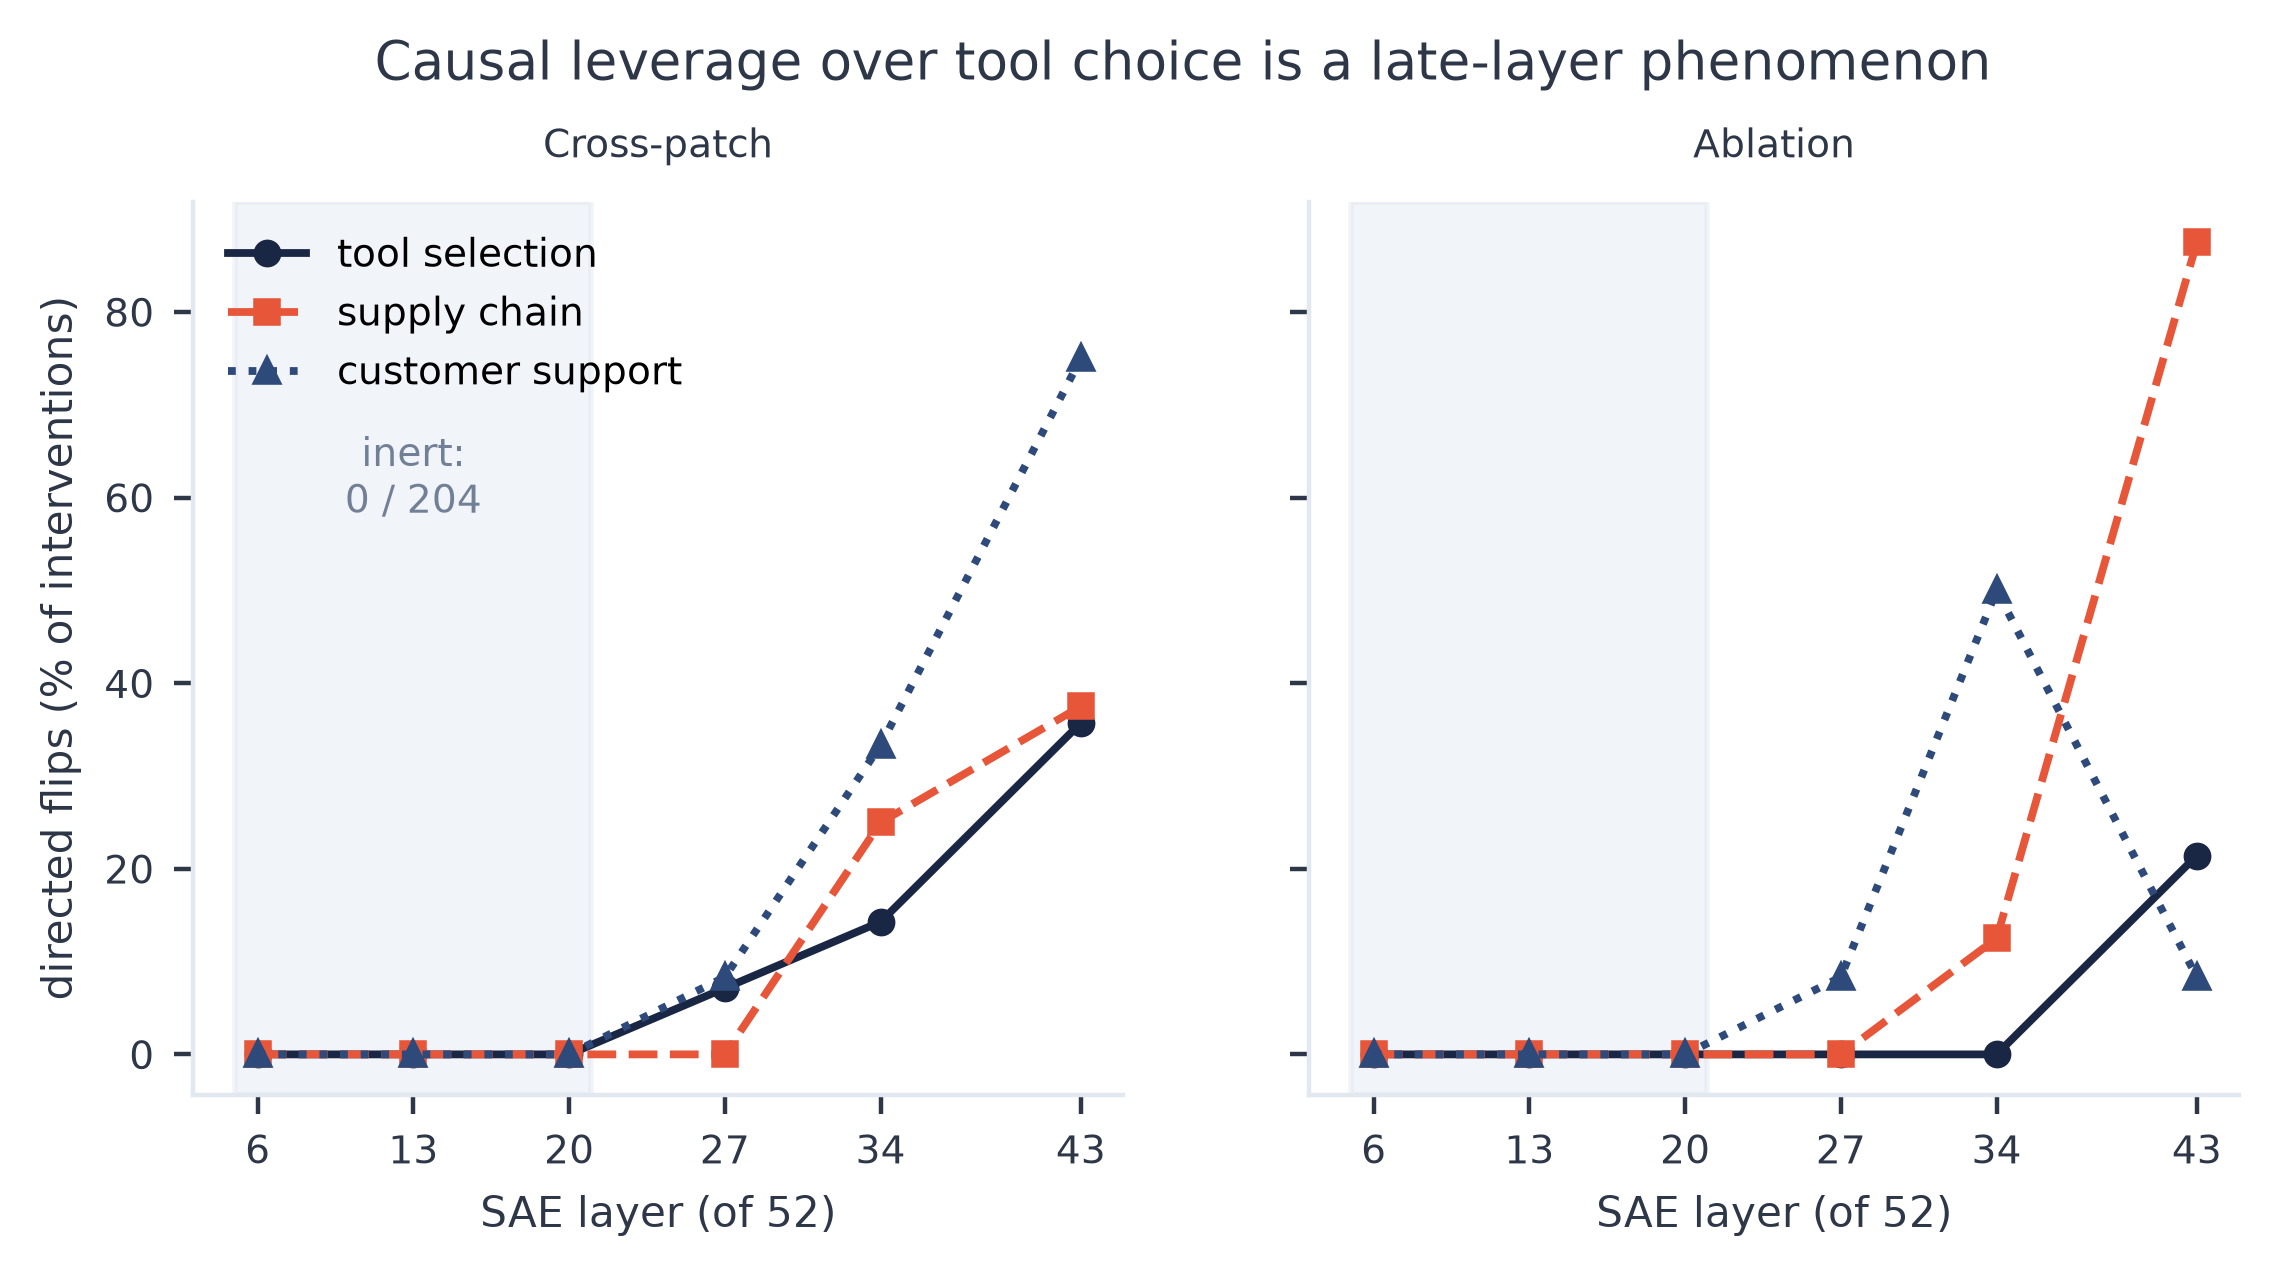
\includegraphics[width=\textwidth]{images/chart_depth.png}
\caption{Directed flip rate against depth, on the demonstration scenarios. Shaded: layers 6--20, where their 204 interventions produce nothing (the expanded sample adds one flip in 256 more; Sect.~\ref{sec:depth}). The customer-support ablation collapse at layer 43 (right panel) is the degeneracy signature of Sect.~\ref{sec:degeneracy}; its inflated cross-patch rate in the left panel is the same artefact seen from the other side.}
\label{fig:depth}
\end{figure}

Early-layer interventions are nearly inert on the evaluated grid. Over layers 6, 13 and 20, the 102 ablation sides and 102 cross-patch directions of the demonstration scenarios produce zero directed flips, with the largest effect anywhere in that region $|\Delta p| = 0.15$ for ablation and 0.09 for cross-patch, against median control thresholds of 0.009--0.050. The expanded sample adds 256 interventions at layer 13 and exactly one flips: a near-tied baseline (0.55 vs.\ 0.43) tipped by $\Delta p = -0.18$ against a control threshold of 0.12. The resulting contrast --- 1 of 460 evaluated early-layer interventions versus 137 of 324 at the primary layers --- is large and consistent across the tested settings, but these dependent counts are not 784 independent trials and do not estimate a model-wide depth effect.

A flip is an argmax crossing, so it depends on where each baseline happens to sit. The same contrast holds on effect size against the strictest control we have. Comparing each cue set with a random set matched on how much it \emph{differs across the pair} --- a quantity with no argmax in it --- the median ratio is $0.81\times$ at layers 6--20 and $2.81\times$ at 27--43, and the cue set clears its band on 21 of 59 early sides against 54 of 68 late ones (Fisher $p = 5 \times 10^{-7}$), counting only genuinely matched draws. Ceiling draws are excluded: their band is the whole eligible pool rather than a matched sample, and they flatter the cue set badly enough to carry the aggregate on their own (28 of 28 late ceiling sides exceed, median $8.77\times$). Early cue sets are, by that measure, not distinguishable from any other set of features that differs as much between the two requests.

This is not because the cue is invisible early. The SAEs at layers 6--20 carry well-labelled features that separate the two sides of a pair; that is exactly what our earlier descriptive analysis at layer 20 reported. In this intervention battery, those features behave as \emph{readouts}: modifying them does not measurably redirect the tool choice.

\paragraph{The same localisation appears along the prompt in these cases.} Depth is one axis; token position is the other (Table~\ref{tab:positions}). At the primary layer, ablating each side's cue features at the \emph{request} tokens moves the decision by at most 0.03 and flips nothing on any of the 20 evaluated sides; ablating them at \emph{every position except the decision token} --- system prompt, tool list, request, chat scaffolding --- also flips nothing; ablating them at the decision token alone changes the tool on 15 of 20 sides, and ablating them everywhere adds essentially nothing to that (max $|\Delta p|$ 0.850 vs.\ 0.847).

Position and depth could in principle trade off against each other: a cue that is inert at the decision token early might still act at the request tokens, which is where an early representation would have to do its work. We ran the same battery at layer 20 to check. It does not: no position set flips any of the 20 sides there, the request tokens included, with the largest movement anywhere 0.151. So the early layers are not merely being intervened on in the wrong place, and the two localisations compose rather than compete. For these prompts and interventions, measurable control is concentrated at one layer range \emph{and} at the position where this model emits its closed-set choice; this does not establish where other models or less constrained decisions are assembled.

\begin{table}[t]
\caption{Ablating cue features at different token positions, at each scenario's primary layer and at layer 20. Cells are \emph{tools changed} / \emph{max} $|\Delta p|$. Depth and position are not separable axes here: at layer 20 no position set moves any decision, including the request tokens, which is where an early-layer cue would have to act if it acted anywhere.}
\label{tab:positions}
\centering
\small
\setlength{\tabcolsep}{5pt}
\begin{tabular}{lcccc}
\toprule
& \multicolumn{2}{c}{Supply chain (8 sides)} & \multicolumn{2}{c}{Customer support (12 sides)} \\
\cmidrule(lr){2-3}\cmidrule(lr){4-5}
Ablated at & L43 & L20 & L34 & L20 \\
\midrule
request tokens          & 0 / 0.007 & 0 / 0.089 & 0 / 0.029 & 0 / 0.111 \\
all but decision token  & 0 / 0.054 & 0 / 0.090 & 0 / 0.244 & 0 / 0.108 \\
decision token only     & \textbf{7 / 0.847} & 0 / 0.053 & \textbf{8 / 0.635} & 0 / 0.151 \\
every position          & 7 / 0.850 & 0 / 0.074 & 8 / 0.744 & 0 / 0.140 \\
\bottomrule
\end{tabular}
\end{table}

The practical consequence within this setting is that \textbf{the layer that gives the most legible feature labels need not be the layer where an intervention changes the decision}. A report built at the former may describe a correlate. Establishing whether this separation recurs in other architectures and tasks requires repeating the layer-wise intervention, not assuming that late-layer localization is universal.

\subsection{Word or meaning?}
\label{sec:semantics}

Cross-patching shows the feature is causal. It does not show what the feature is \emph{about}. Two probe families separate the cue's meaning from its surface form.

Keyword probes hold in 9 of 12 cases: inserting the cue word into the other side's request in a semantically inert role usually leaves the tool alone. \emph{``Adjust inventory for items with rising customer order frequency, using the cost codes from the forecasted budget approved last week''} stays on \texttt{inventory\_manager}. All five customer-support probes hold. Two of the three failures fall on \emph{cost vs.\ speed}, the pair independently flagged as weak in Sect.~\ref{sec:limitations}.

Paraphrases hold in 30 of 40 cases. The failures are informative: \emph{``projected to rise''} keeps the forecast reading, \emph{``expected to be ordered more often in the period ahead''} does not. So the feature is not a token detector --- but neither is it \emph{forecasting} in general. It tracks a fairly narrow sense of \emph{forecast framing of the demand signal}. We think this is the right level of claim to make about a single SAE feature on present evidence, and note that stronger claims are easy to make accidentally when only positive probes are reported.

\paragraph{Directionality.} Steering is asymmetric. \emph{Local vs.\ global sourcing} flips $a \to b$ at $1\times$ ($p = 0.12 \to 0.75$) but in the other direction only reaches $p = 0.50$ at $3\times$, without ever changing the tool; \emph{urgent vs.\ routine} flips $b \to a$ at $1\times$ and does not move at all the other way ($0.01 \to 0.05$ at $3\times$). Adding a reading is consistently easier than removing one --- which is what one would expect if the cue features add evidence for a tool rather than gating it.

\section{When SAE Features Are Not Usable: A Degeneracy Diagnostic}
\label{sec:degeneracy}

The starred cell in Table~\ref{tab:depth} looks like the best result in the study. Customer support at layer 43 flips 9 of 12 cross-patch directions --- better than any other cell. It is in fact the one cell where nothing can be concluded, and the way it fails is general enough to be worth a diagnostic.

\subsection{The dictionary has collapsed}

At layer 43 the customer-support prompts activate a mean of 1{,}167 features --- against a training target $L_0$ of 75 --- of which \textbf{1{,}162 fire on every one of the twelve prompts} and only 32 vary at all. The cleanest statement of the problem is per pair: the median number of features active on one side of a pair and \emph{not} on the other is \textbf{1}, and for one side it is 0. There is nothing left for a cue analysis to name. The same scenario at layer 34 gives a median of 13 side-specific features on a mean $L_0$ of 73, and supply chain at layer 43 gives 5 on an $L_0$ of 32 --- so this is a property of this input distribution meeting this dictionary, not of the layer alone (Table~\ref{tab:health}). Tool selection makes the point sharper still: on the \emph{same} layer-43 dictionary its prompts activate a mean of 374 features, five times the target, and it remains perfectly usable, retaining 22 side-specific features per pair and producing 3 ablation and 5 cross-patch flips. Density is not the failure; the disappearance of the difference between two sides of a pair is.

\begin{table}[t]
\caption{Dictionary health at the two deepest layers. \emph{Always on} counts features active on every prompt of that scenario, with its share of the active code in brackets; \emph{side-specific} is the median number active on one side of a pair and not the other. Explained variance is highest exactly where the decomposition is least usable. The tool-selection rows are the informative complication: that scenario runs at 5--8$\times$ the target $L_0$ at both layers and is still usable, because what collapses is the side-specific column, not the density column.}
\label{tab:health}
\centering
\small
\setlength{\tabcolsep}{5pt}
\begin{tabular}{@{}llrrrr@{}}
\toprule
Scenario & Layer & Mean $L_0$ & Expl.\ var. & Always on & Side-specific \\
\midrule
Supply chain     & 34 & 36 & 0.62 & 2 (0.01) & 18 \\
Supply chain     & 43 & 32 & 0.73 & 16 (0.18) & 5 \\
Tool selection   & 34 & 633 & 0.52 & 222 (0.20) & 69 \\
Tool selection   & 43 & 374 & 0.66 & 219 (0.42) & 22 \\
Customer support & 34 & 73 & 0.68 & 42 (0.19) & 13 \\
Customer support & 43 & \textbf{1{,}167} & \textbf{0.86} & \textbf{1{,}162 (0.97)} & \textbf{1} \\
\bottomrule
\end{tabular}
\end{table}

Under those conditions the \textsc{bulk} cross-patch stops being an intervention on features and becomes a transplant of the whole representation. Splitting the nine flips accordingly: \textbf{one} comes from the cue families; the other eight require clamping all $\sim$1{,}163 base-active features. The comparison cells are unambiguous --- supply chain at layer 43 gets 3 of 3 flips from cue families with a median of 22 features clamped, tool selection 2 of 5 with 352, customer support at layer 34 2 of 4 with 48.

\subsection{Reconstruction quality points the wrong way}

The natural instinct is to catch this with a quality metric. It does not work. Figure~\ref{fig:degen} (left) plots explained variance per layer: customer support at layer 43 scores \textbf{0.86, the highest value anywhere in the study}, well above the layers that actually steer (supply chain 43: 0.73; customer support 34: 0.68). A dictionary that reconstructs the residual stream almost perfectly by keeping 1{,}162 features permanently on is doing exactly what a reconstruction objective asks of it. Raw $L_0$ is a better hint, and a weaker one than it looks. This dictionary already misses its sparsity target on its own training data --- mean $L_0$ 557 against a target of 75, median 374, 95th percentile 1{,}168 across 200 batches --- so the 1{,}167 we measure on the customer-support prompts is not an out-of-distribution pathology but the top of the range the dictionary already occupied, and the 374 on the tool-selection prompts is exactly its training median. A threshold on $L_0$ that fires on the first would have to fire on a great deal else. $L_0$ is in any case a property of the dictionary in the abstract, measured before any intervention, and it gives no reading on the specific analysis being attempted.

\begin{figure}[t]
\centering
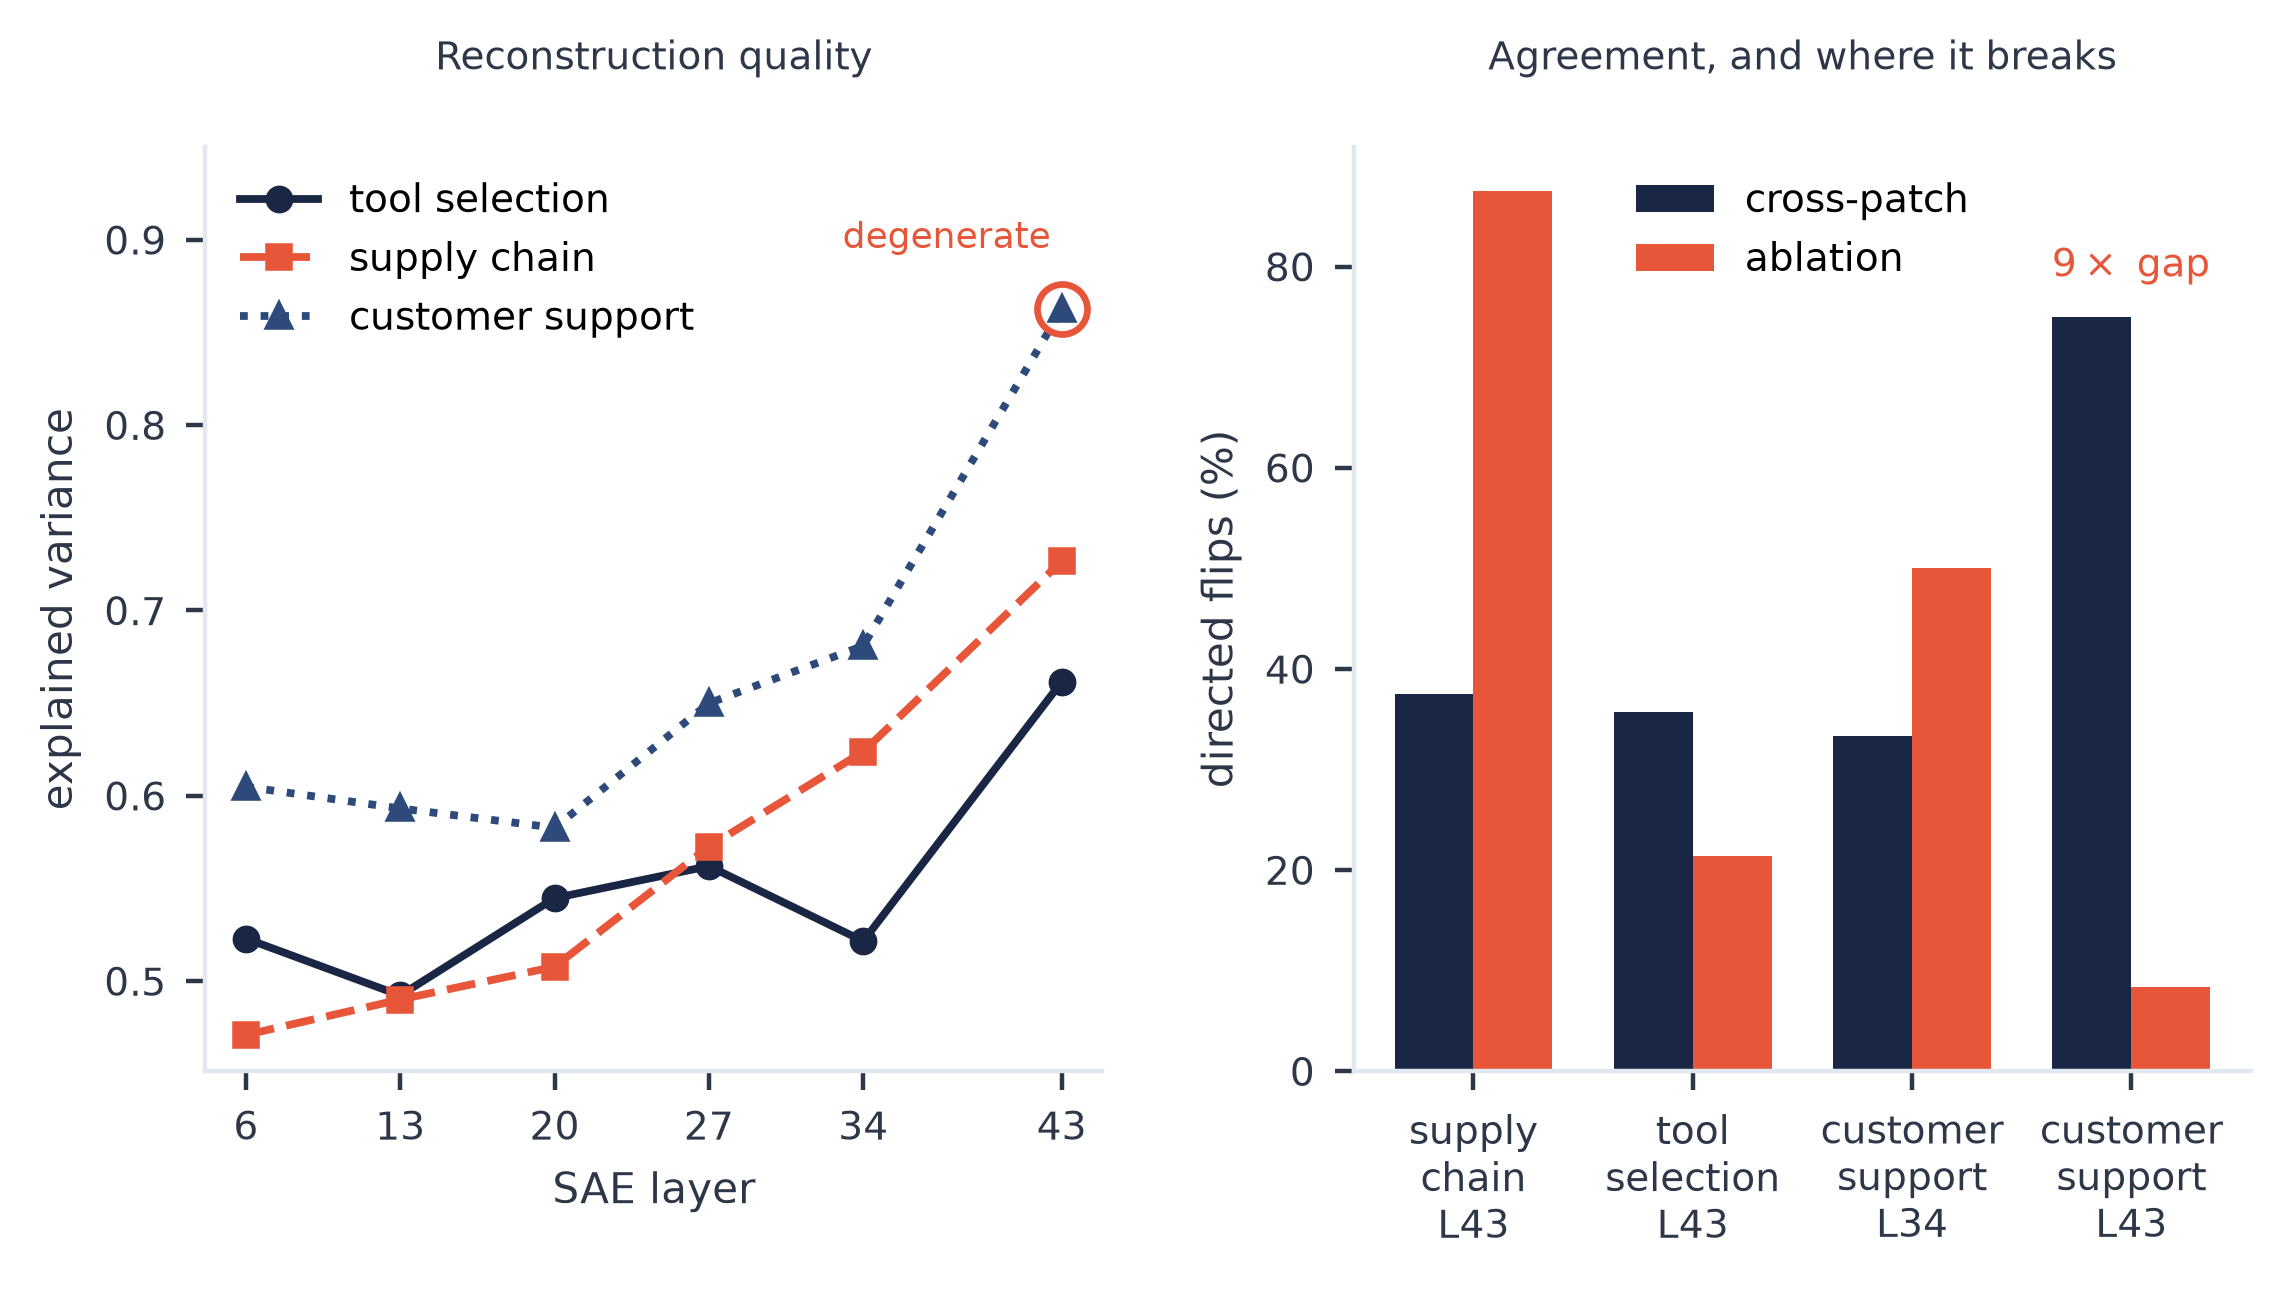
\includegraphics[width=\textwidth]{images/chart_degeneracy.png}
\caption{Left: explained variance peaks exactly where the dictionary is unusable --- the circled point is customer support at layer 43, mean $L_0$ 1{,}167 with 1{,}162 of those features active on every prompt. Right: cross-patch and ablation flip rates stay within a factor of 2.5 on healthy cells and diverge by a factor of 9 on the collapsed one.}
\label{fig:degen}
\end{figure}

\paragraph{Two cheap signals that do work.} Explained variance points the wrong way and $L_0$ is unreliable, but two statistics computed on the analysis's own inputs --- before any intervention --- separate the collapsed cell cleanly. The share of the active code that fires on \emph{every} prompt is 0.97 for customer support at layer 43 against at most 0.42 anywhere else in the grid, and the median count of side-specific features per pair is 1 against 5--69 (Table~\ref{tab:health}). Neither costs a forward pass beyond the capture the analysis already requires, and neither is fooled by density alone, which is what separates them from $L_0$. We state them first because they are the cheapest thing that works: a section arguing that a metric should be chosen on whether it detects the failure would be poorly placed to recommend only its own.

\subsection{The diagnostic: cross-patch and ablation should stay close}

Ablation and cross-patch probe opposite directions of the same claim --- necessity and sufficiency of the same feature set --- so their flip rates should be of comparable size, in whichever order. On the three healthy cells they are, within a factor of 2.5 (Fig.~\ref{fig:degen}, right): supply chain 43 gives 37\% cross-patch against 88\% ablation ($2.4\times$), tool selection 43 gives 36\% against 21\% ($1.7\times$), customer support 34 gives 33\% against 50\% ($1.5\times$). The collapsed cell gives 75\% against 8\% --- a factor of \textbf{9}.

That gap is mechanically what collapse predicts, which is why it is a diagnostic and not a coincidence. Cross-patching is inflated because the transplanted set is the whole prompt rather than a cue. Ablation is deflated because removing six cue families out of 1{,}167 active features changes almost nothing. Neither rate is informative on its own; the ratio between them is.

We therefore propose \textbf{the cross-patch/ablation ratio as a second, intervention-native screen} alongside the two input-side statistics above. Its case is not that it is more sensitive --- on our grid the always-on share is at least as sensitive and far cheaper --- but that it is measured on the intervention actually being made rather than on the dictionary or the activations in the abstract, so it can fail for reasons an input-side statistic cannot see: a code that varies plentifully across a pair may still be one whose variation does not carry the decision. It costs one extra battery over an experiment already being run. In this study it separates the one unusable cell from the five others where it is defined, and it is what moved the customer-support analysis from layer 43 to layer 34.

\paragraph{The screen needs a minimum count.} The ratio exists only where the ablation arm flips at least once, which is 6 of the 18 cells in our grid. Ten of the other twelve produce no flips in either arm and say nothing at all. The remaining two --- tool selection at layers 27 and 34, with 1 and 2 cross-patch flips against 0 ablation flips --- carry the arithmetic signature of collapse, an unbounded ratio, at counts far too small to read; and their dictionaries are dense (mean $L_0$ 353 and 633) without being collapsed in the sense that matters, retaining 52 and 69 side-specific features per pair. A screen that reported those two as failures would be wrong about both. So the precondition belongs to the diagnostic rather than beside it: do not read the ratio below roughly five flips in the ablation arm, and read a zero-ablation cell as \emph{uninformative} rather than as collapsed.

We state the obvious caveat: one collapsed cell is an existence proof, not a calibration. The factor-of-2.5 boundary is where our cells happen to fall, not a threshold we have validated, and a diagnostic built on 17 pairs in one model should be treated as a cheap smoke test rather than a certificate.

\section{Limitations}
\label{sec:limitations}

\paragraph{Scale and correlation of the pair sets.} The demonstration sets (34 sides) establish existence, and the expanded sample (128 sides) gives exploratory rates for \emph{two scenarios in one model}, not for tool selection in general. Within a contrast type the generated pairs are near-duplicates, so the effective sample is smaller than 128. Our contrast-cluster bootstrap preserves that dependence and yields wide intervals (ablation 0.42--0.66; cross-patch 0.16--0.48), but only ten clusters are available, so it cannot support precise generalization. The selection rules, seeds, gate population, and bootstrap code are published with the pairs.

\paragraph{The dictionaries have seen the evaluation distribution.} The SAEs are trained on decision-token activations from the same generated corpus the evaluation pairs are drawn from, and 136 of the 150 evaluated requests appear in it verbatim (Sect.~\ref{sec:method}). This does not weaken the causal reading of any individual intervention --- a cross-patch either changes the tool or it does not, and its controls are drawn under identical conditions --- but the reported \emph{rates} are in-distribution for the dictionary, and a feature vocabulary fitted on these prompts may decompose them more cleanly than it would decompose unseen ones. Sect.~\ref{sec:heldout} probes this on contrast types absent from the training corpus; the probe is small, and a fuller answer needs dictionaries trained with a held-out split reserved in advance.

\paragraph{One model, one SAE suite, and one decision form.} All results are from NVIDIA Nemotron 3.5 Nano, a single 52-layer hybrid that interleaves Mamba-2, attention, and mixture-of-experts blocks, using one release of SAEs trained on its residual stream. The depth result is therefore local: causal leverage concentrates at layers 34 and 43 for the evaluated tool-selection prompts and interventions. We cannot distinguish whether this pattern reflects this architecture's division of labour, a broader tendency of large models to consolidate decisions late, or the closed-set and discrete nature of tool selection. It should not be read as a universal claim about where language models make decisions. Two properties of this architecture give concrete reasons to expect it may localise differently from the dense transformers the SAE literature is built on, which we offer as hypotheses rather than findings. Mixture-of-experts routing means the residual stream the dictionaries were fitted on pools prompts that took different expert paths, so one dictionary describes a union of routing regimes rather than a single one --- a plausible contributor to the layer-43 density of Sect.~\ref{sec:degeneracy}. And Mamba-2 blocks carry information along the sequence in a recurrent state rather than by attending to particular positions, which could spread cue information across positions differently from a model where a cue token is attended to directly; that bears on Table~\ref{tab:positions}, which we measure at one layer in one architecture. Testing the depth claim requires comparable layer-wise interventions across architectures, SAE suites, model scales, and open-ended as well as closed-set tasks. The degeneracy diagnostic is architecture-agnostic in its definition, but its usefulness elsewhere remains a conjecture.

\paragraph{The primary layer is the argmax of the grid we report.} Layers 43 (supply chain, tool selection) and 34 (customer support) were not chosen independently of the results: they are the most responsive of the six evaluated layers, selected on the same demonstration battery that Table~\ref{tab:depth} reports. Table~\ref{tab:expanded} should therefore be read as flip rates \emph{at the most responsive of six evaluated layers}. The margins are wide --- 7 combined flips over the runner-up for supply chain, 6 for tool selection --- and for customer support the choice was made by the degeneracy diagnostic rather than by count, since layers 34 and 43 tie at 10 combined flips and 43 is the collapsed cell. The selection is nonetheless real, and it inflates the headline rate. Layer 27, which no selection step touched, gives 20 of 128 ablation flips and 15 of 128 cross-patch on the same expanded pairs, against 68 and 41 at the selected layers --- a factor of $3.4$ and $2.7$. What the selection buys is effect size, not the depth pattern itself: substituting layer 27 for the primary layers leaves the early-versus-late contrast of Sect.~\ref{sec:depth} intact at 1 of 460 against 38 of 324 (Fisher $p = 2 \times 10^{-14}$).

\paragraph{Cue families are chosen by contrast, not by circuit.} We intervene on the features that differ across a pair. That is the right set for the question we ask, but it is not a circuit: we do not identify what writes those features upstream, nor what reads them downstream. The 27-to-43 transition, where the same features go from inert to decisive, is the obvious place to look and we have not looked.

\paragraph{Weak pairs remain weak.} \emph{Cost vs.\ speed} fails on three independent signals --- wide control bands (set-matched, 0.12--0.19), no ablation flip on side A, no cross-patch flip in either direction --- and two of the three keyword-control failures fall on it. We report it rather than dropping it, but it carries no weight. \emph{Single issue vs.\ complex case} is not a true minimal pair either: side B is side A plus an appended list, so its contrast is partly length.

\paragraph{Behaviour beyond the decision token is barely tested.} The generation arm is 20 directions, of which 5 move the decision token; all 5 carry into the first tool named in 48 generated tokens, and no control does. That is the right conditional, but it rests on five events, and 48 tokens establish only that the first named tool changes. Whether an agent would carry the changed plan through a multi-step episode --- a retrieval, a tool result, a second decision --- is untested, and it is the first question anyone intending to use this for control would ask. We report the generation arm as evidence that the effect reaches behaviour at all, not as evidence about behaviour at length.

\section{Conclusion}
\label{sec:conclusion}

Sparse autoencoder features on the evaluated agentic model are not only describable but can be causally effective. In our clearest case, a single feature clamped into an unmodified request at a naturally occurring value changes which tool the model calls, moves its probability from 0.15 to 0.71, exceeds its mass-matched controls, and changes what the model writes. Effective is not the same as sufficient: against a ceiling that patches the whole residual at that token, cue-set interventions recover 29\% of the available causal signal, and a dense direction of equal magnitude recovers the same share --- so what the sparse basis contributes is an intervention that can be named, not one that reaches further. The expanded evidence supports causal effects from small cue-feature sets rather than establishing that single-feature control is typical. Across this model's evaluated layer grid, comparable leverage is almost absent early even though the cues are cleanly represented there, so an explanation built where features are most legible may describe a correlate rather than a cause of the decision. Whether this late concentration generalizes beyond this hybrid architecture and closed-set tool-selection task remains open.

The negative result is the one we would most like carried forward. The single cell in our grid where the SAE could not support any causal claim is also the cell with the best reconstruction. What separates it is not reconstruction quality but how much of the code still varies across the inputs being compared --- 97\% of its active features fire on every prompt, and the median pair leaves one feature that distinguishes the two sides --- and, as a second check measured on the intervention itself, whether the cross-patch and ablation rates are the same size. As SAEs move into production explainability, screens of that kind should be a precondition for the claim, not an afterthought.

% References, acknowledgments, and the checklist do not count toward the
% nine-page NeurIPS main-content limit.
\clearpage

\begin{ack}
We thank the 575 Lab team at Dataiku. Run artefacts, selection rules,
interactive per-pair reports, and the code to reproduce every figure are
available in the project repository.
\end{ack}

\bibliographystyle{plainnat}
\bibliography{references,steering_refs}

\input{checklist}

\end{document}
